\documentclass[a4paper,12pt]{article}
\usepackage{graphicx}
\usepackage{epsfig}
\usepackage{amsmath}
\usepackage{color}
\usepackage{ifthen}

\makeatletter
\newenvironment{tablehere}
{\def\@captype{table}}
{}
\newenvironment{figurehere}
{\def\@captype{figure}}
{}
\makeatother

\newcommand{\hideAnswers}{0}

\newcommand{\answerbox}[1]{
\ifthenelse{\hideAnswers = 1}{%
}{%
{\mbox{}\\{{\color{blue}\it\mbox{}#1}\color{black}}}%
}}

\title{EM Homework 1}
% \author{To be handed in by Friday, Week 18, 2pm.\\
% Problems will be discussed in tutorials Week 19.}

\date{}
\renewcommand{\labelenumi}{\arabic{enumi}.)} % 1,2,
\renewcommand{\labelenumii}{\alph{enumii}.)} % a,b,
\renewcommand{\labelenumiii}{\roman{enumiii}.)} % i, ii

\begin{document}

\maketitle

%Please hand in the answers to these questions before meeting your tutor.

\begin{enumerate}

\item  For the arrangement of charges shown in the diagram below, calculate:

  \begin{figure}[!!h]
    \begin{center}
      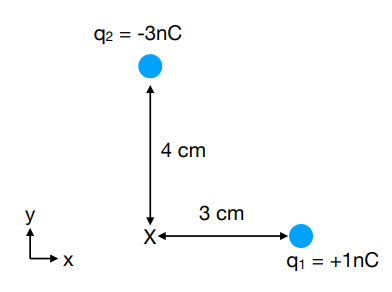
\includegraphics[width=0.5\textwidth]{HW1_chargePic}
    \end{center}
  \end{figure}

	\begin{enumerate}
	\item the Coulomb force between the two charges
	
	 \answerbox{The distance between the charges can be found from $r = \sqrt{3^2 + 4^2}$ cm $= 5$ cm,  so:
	 
	 \begin{align*}
		F &= \frac{q_1 q_2}{4 \pi \epsilon_0 r^2} \\
		&= \frac{1 \times 10^{-9} \cdot -3 \times 10^{-9} }{4 \pi \cdot 8.85 \times 10^{-12} \cdot 0.05^2} \\
		&= -1.1 \times 10^{-5} \text{N} 	 
	 \end{align*}
	 
	 The answer is negative, so this is an attractive force.
}
	 
	\item the electric field at point X.
	
	\answerbox{ We have to find the field due to $q_1$ and $q_2$ individually, then take the
vector sum.
	\begin{align*}
	E_1 = \frac{q_1}{4 \pi \epsilon_0 r^2} = 9 \times 10^9 \frac{1 \times 10^{-9} }{0.03^2} = 10^4 \text{Vm}^{-1}
	\end{align*}
	
	\noindent where $\frac{1}{4 \pi \epsilon_0} = 9 \times 10^9$. The $\mathbf{E}_1$ vector points away from $q_1$ (negative $x$-direction).   

	\begin{align*}
	E_2 = \frac{q_2}{4 \pi \epsilon_0 r^2} = 9 \times 10^9 \frac{-3 \times 10^{-9} }{0.04^2} = -1.69 \times 10^4 \text{Vm}^{-1}
	\end{align*}	
	
	The $\mathbf{E}_2$ vector points towards $q_2$ (positive $y$-direction). \\
	
	$\mathbf{E}_1 = -10^4 \hat{\mathbf{i}}$ and $\mathbf{E}_2 = 1.69 \times 10^4 \hat{\mathbf{j}}$, hence $\mathbf{E} = -10^4 \hat{\mathbf{i}} + 1.69 \times 10^4 \hat{\mathbf{j}}$. \\
	
	The overall magnitude of the $E$-field at point X is: \\
	
	$E_X = \sqrt{(-1 \times 10^4)^2 + (1.69 \times 10^4)^2} = 1.96 \times 10^4$ Vm$^{-1}$. The direction of the field is $\tan^{-1} \left( \frac{E_y}{E_x} \right) = -59^{\circ}$ ($59^{\circ}$ above the negative $x$-axis.) 
	
	}
	
	\item the force on a 3rd charge, of -2nC, placed at point X.
	
	\answerbox{The magnitude of the force on a -2 nC charge placed at point X is given by: 
	\begin{align*}	
	F &= qE_X \\
			&= 2 \times 10^{-9} \cdot 1.96 \times 10^4 \\
			&= 3.92 \times 10^{-5} \text{N}   
	\end{align*}

\noindent The direction of the force will be in the opposite direction to the total field at that point (i.e., 58$^{\circ}$ below the positive $x$-axis). 
	}
	
	\end{enumerate}
	
	
\item Draw the electric field lines of a system consisting of:
	\begin{enumerate}
	\item two charges of equal magnitude and same sign. \\
	
	  \begin{figurehere}
    \begin{center}
      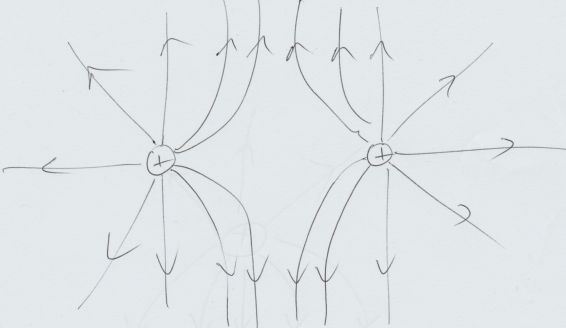
\includegraphics[width=0.7\textwidth]{HW1_2a}
    \end{center}
  \end{figurehere}
	
	
	\item two charges of equal magnitude, but opposite sign. \\
	
	
	  \begin{figurehere}
    \begin{center}
      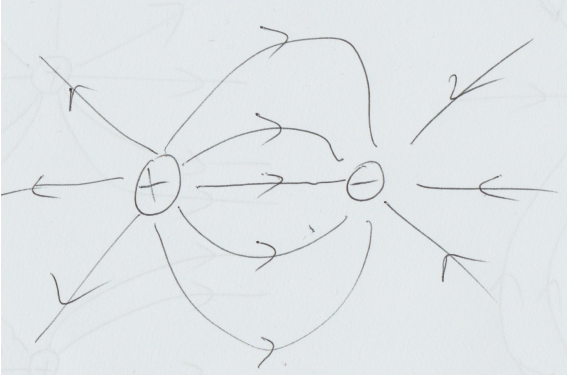
\includegraphics[width=0.7\textwidth]{HW1_2b}
    \end{center}
  \end{figurehere}
	
	
	\item one charge of -5C and one of +3C. \\

	  \begin{figurehere}
    \begin{center}
      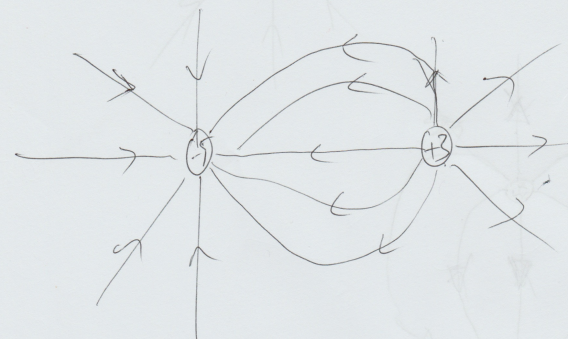
\includegraphics[width=0.7\textwidth]{HW1_2c}
    \end{center}
  \end{figurehere}
	
  	\end{enumerate}

\noindent In general, the rules that must be followed are: 
\begin{itemize}
\item field line density higher close to charges, i.e. more coming from/arriving
on largest charge.
\item all field lines from smaller charge connected to larger charge; larger charge has some spare ones (these go to infinity).  
\item arrows in right direction; start on pos charge, end on negative
charge.
\end{itemize}

\newpage

\item Look at the circuit below.
  The switch $S_1$ is closed and the capacitor uncharged. 
  \begin{figure}[!!h]
    \begin{center}
      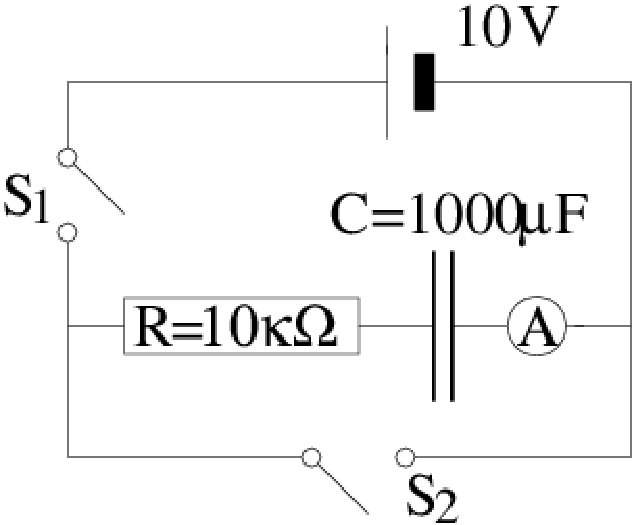
\includegraphics[width=0.3\textwidth]{cap_circ3.pdf}
    \end{center}
  \end{figure}
  \begin{enumerate}
  \item Calculate the current measured in the Ammeter
    immediately after closing $S_1$.
	
    \answerbox{
    At the moment of closing the 10~$V$ potential difference is all of a sudden over the RC-system. 
       $\Delta V$ over the capacitor is still zero, so the whole 10~$V$ drop over the resistor.
       Hence, 
       \begin{equation}
         I=\frac{V}{R}=\frac{10V}{10\cdot 10^3 \Omega}=1~mA
       \end{equation}
    }   
	
  \item Calculate the current measured in the Ammeter
    10~$s$ after closing $S_1$.
	 
	 \answerbox{
	   When charging a capacitor, the current changes as:\\ 
	      $ I(t) = I(0) e^{-\frac{t}{RC}} = 1mA \cdot e^{-\frac{10s}{10^4\Omega \cdot 10^-3 F}} = 0.37 mA$.\\
  
	Alternatively, you can calculate the voltage over the resistor after 10s and obtain the current that way.
	The voltage over the capacitor is given by the charging up equation. Putting in the numbers
	    \begin{equation}
	      V_C=V_0\left(1-e^{-\frac{t}{RC}}\right)=10\left(1-e^{-\frac{10s}{10s}}\right)=6.3~V
	    \end{equation}
	    Thus there falls $10.0V-6.3V=3.7~V$ over the resistor. Using Ohm's Law $I=V\Big/R=3.7 V \Big/ 10\cdot 10^3 \Omega=0.37~mA$. \\
    

	 } 
	
  \item Calculate the current measured in the Ammeter
    5 minutes after closing $S_1$.\\
    \answerbox{
        5 minutes are so long compared to the $RC=10~s$ time interval that the capacitor is essentially charged up to 
     $10~V$. So there is no potential difference across the resistor and thus the current is zero.\\
    } 
    
    After 10 minutes the switch $S_1$ is opened and $S_2$ is closed.
  \item Calculate the current measured in the Ammeter
    immediately after closing $S_2$.
	
    \answerbox{
        So now the voltage source is no longer connected by the current now comes from the discharging of the capacitor.
     At the moment of closing the voltage over the capacitor is still 10~$V$. Thus using Ohm's law
     we find again 1~$mA$.
    } 
	
  \item Calculate the current measured in the Ammeter
    10~$s$ after closing $S_2$.
	
    \answerbox{
     Also when discharging the capacitor, the current changes exponentially accoring to:\\
        $ I(t) = I(0) e^{-\frac{t}{RC}} = 1mA \cdot e^{-\frac{10s}{10^4\Omega \cdot 10^-3 F}} = 0.37 mA$.\\
    As the voltage source is no longer connected the voltage over the capacitor is the same as the voltage over the resistor (resistance in ammeter is neglibible).
    }   
	
  \item Calculate the current measured in the Ammeter
    5 minutes after closing $S_2$.
	
    \answerbox{
        5 minutes after closing $S_2$.\\
    After such a long time the discharging is essentially complete. So no voltage drop over the resistor,
    hence no current is flowing.
    }
	
  \end{enumerate}


\end{enumerate} % end of homework


\end{document}
